% ------------------------------------------------------------------------------
%
% PREAMBLE
%
% ------------------------------------------------------------------------------

\documentclass[12pt, titlepage]{article}


\usepackage{graphicx, amsmath, amssymb, natbib, setspace, sectsty, verbatim, 
		mathrsfs, float}
\usepackage{MnSymbol}
\usepackage{multirow}
\usepackage{bm}
\usepackage[usenames, dvipsnames]{color}
\bibpunct{(}{)}{;}{a}{}{,}
\setlength{\parindent}{3em}
%\parskip = 1.5ex
%\linespread{1.3}
%\onehalfspacing

\pdfpagewidth 8.5in
\pdfpageheight 11in
\setlength{\oddsidemargin}{0.0in} \setlength{\textwidth}{6.5in}
\setlength{\topmargin}{0.15in} \setlength{\textheight}{8.5in}
\setlength{\headheight}{0.0in} \setlength{\headsep}{0.0in}

\usepackage{/mnt/ExtraDrive1/Work/shTex/mymacros}

\providecommand{\norm}[1]{\lVert#1\rVert}
\newcommand{\csection}[1]{\section[#1]{\centering #1 }}
\subsectionfont{\small}
\newcommand{\cye}[1]{\color{yellow!70!black}#1}
\newcommand{\cre}[1]{\color{red!70!black}#1}
\newcommand{\cbl}[1]{\color{blue!70!black}#1}
\newcommand{\cgr}[1]{\color{green!70!black}#1}


% ------------------------------------------------------------------------------
%
% BEGIN DOCUMENT
%
% ------------------------------------------------------------------------------

\begin{document}

\setcounter{equation}{0}
\renewcommand{\theequation}{R.\arabic{equation}}


% ------------------------------------------------------------------------------
%
%                    Section 8.8.1
%                    Seal trend data
%
% ------------------------------------------------------------------------------

{\large \flushleft \textbf{9.11.3 Moss Heavy Metal Data}}

\vspace{.3cm}

In Section 8.7.4, we used a spatial linear model for the logarithm (base $e$) of lead (Pb) concentration in tissue samples that included explanatory variables for 1) year of sample (2001 or 2006), 2) (log, base $e$) distance-from-road, and 3) side-of-road (north or south).  We fit a mean structure where the dominant effect was distance-from-road. There also appeared to be some lowering of Pb concentration in 2006 due to better coverings on trucks that transported ore on the haul road, although the P-value of 0.118 would be judged nonsignificant if our critical values were $\alpha = 0.05$ or $\alpha = 0.10$. 

In prior examples in this Chapter, for the wet sulfate data and harbor seals, we used kriging and spatial prediction to make maps with point-wise or polygon-wise predictions with standard errors (mean-squared prediction errors) of those predictions.  In this Section we will focus on conditional simulation for the heavy metal data.  We have 5 prediction data sets, and they are shown as stratum 1 through stratum 5 in Figure 1.8B.  Recall that the data are modeled after a log transformation, but we wish to make inferences back on the natural scale of the data.  This nonlinear back-transformation, coupled by any further computations on a whole prediction surface, complicates the construction of the covariance matrix for predictions.  Rather, we simulate a whole surface on the transformed scale, then back-tranform that whole surface, and then perform further computations.  Because we simulate many equal-probable surfaces, we perform our inference \textit{after} computing on individual surfaces by using the variation among the computed values on individual surfaces.

As an example, consider whether or not there is a difference between 2001 and 2006 in each stratum for the moss heavy metal data.  First, we simulate a surface using conditional simulation, with fixed effects set at 2001 and 2006 (so we essentially simulate the surface twice, but with the same set of fixed effects and covariance parameters).  Then, we exponentiate the values comprising the surface, average the 2001 and 2006 surfaces, and then take the averaged 2001 surface minus the 2006 surface.  Trying to find the variance of this difference would be quite difficult based on our original model on the log scale.  However, using conditional simulation, we simply simulate another surface, and repeat all computations.  

For our example, we did this 500 times, and a histogram of the differences between 2001 and 2006 are shown in Figure~\ref{Fig:MossDiffHist}.  Notice that for strata 1 through 4, there is very strong evidence that Pb concentrations went down from 2001 to 2006, as all computations from 500 conditional simulation showed positive values.  To estimate P-values, we can use quantiles from the simulations.  Here, because all 500 simulations are greater than 0, we can state that P < 0.002. The histograms of these differences have a Gaussian shape, so we are also justified in using a normal distribution approximation by taking the mean of differences divided by the standard deviation of the differences.  Doing so estimates that P < $10^{-5}$ for all strata.  Strata 5 is a control, being far to the south from the road, and here we see a nonsignificant difference between 2001 and 2006.  If we order the differences, then 67 differences are less than 0 and 433 are greater than 0, so a two-tailed P-value is 2*(1 - 67/500) = 0.268.  Using the normal approximation we obtain P = 0.403.

\begin{figure}[H]
  \begin{center}
	    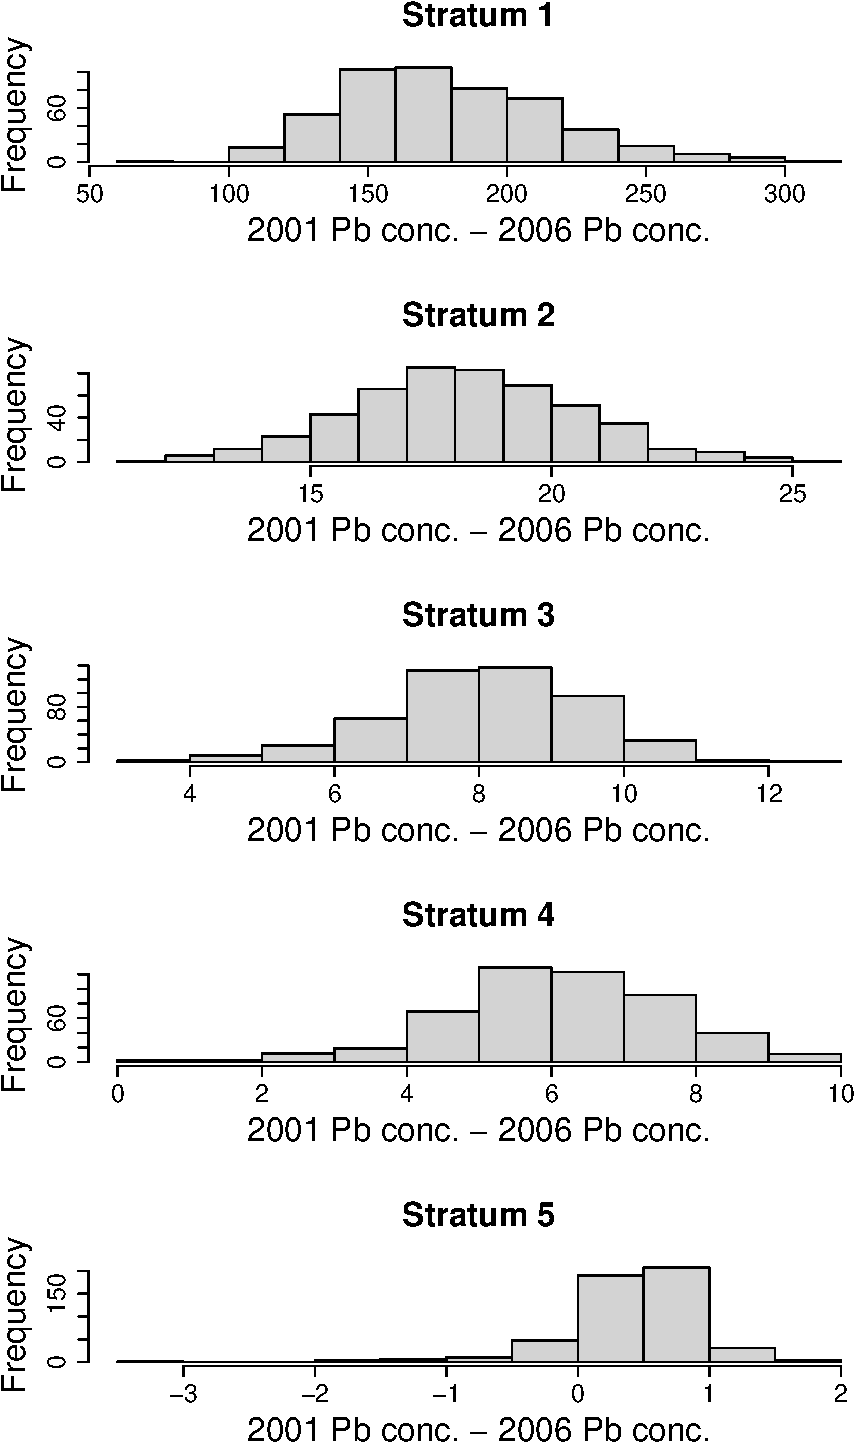
\includegraphics[width=0.5\linewidth]{Moss_diffhist}
  \end{center}
  \caption{Histograms of the difference between 2001 and 2006 average Pb concentrations per stratum. \label{Fig:MossDiffHist}}
\end{figure}

Using conditional simulation, we have very strong evidence that Pb concentrations were lower in 2006 than 2001, and because the control (stratum 5) did not change significantly, we can conclude that the coverings on the trucks decreased the contamination of Pb near the haul road.  Recall that in Chapter 8, when we fit this model, while the intercepts were different between 2001 and 2006, the P-value was greater than 0.10, so that difference was not conclusive.  Why is the evidence here, using conditional simulation, so much stronger?  The reason is that in Chapter 8, we were making an inference on a mean parameter in a model, while here we are making an inference on predictions of what was actually realized in nature.  This is an important distinction that we should always keep in mind.  Do we want to make an inference on the mean of some statistical process that produced the observed data, where the data may actually be quite far from that mean, or do we want to make an inference on those realized data?  More simply, do we want to make an inference on what would happen on average if we let time start over again and our model was correct, or do want to make an inference on what actually happened.  There is no right answer, and it depends on how broadly you want your inference to apply. Notice that this may seem somewhat confusing, as we are using conditional simulation to create equal-probable surfaces, but the key word here is ``conditional,'' as those equal-probable surfaces are constrained by the observed data.

For example, the mean, on the log scale, 




%%%%%%%%%%%%%%%%%%%%%%%%%%%%%%%%%%%%%%%%%%%%%%%%%%%%%%%%%%%%%%%%%%%%%%%%%%%%%%%%
%%%%%%%%%%%%%%%%%%%%%%%%%%%%%%%%%%%%%%%%%%%%%%%%%%%%%%%%%%%%%%%%%%%%%%%%%%%%%%%%                BIBLIOGRAPHY
%%%%%%%%%%%%%%%%%%%%%%%%%%%%%%%%%%%%%%%%%%%%%%%%%%%%%%%%%%%%%%%%%%%%%%%%%%%%%%%%
%%%%%%%%%%%%%%%%%%%%%%%%%%%%%%%%%%%%%%%%%%%%%%%%%%%%%%%%%%%%%%%%%%%%%%%%%%%%%%%%

%\bibliographystyle{consbiol}
\bibliographystyle{/mnt/ExtraDrive1/Work/shTex/asa}
\bibliography{DaleChap884.bib}
%\bibliographystyle{/home/jay/Data/shTex/shTex/asa}
%\bibliography{/home/jay/Data/shTex/shTex/StatBibTex.bib}




\end{document}

